We evaluate \checkcell{} across two dimensions: its execution time,
and its effectiveness at finding actual errors.

Our experimental platform is a 13'' MacBook Air equipped 4GB of RAM
and an Intel Core i5-2557M processor running at 1.70GHz. The operating
system is Windows 7 Professional (SP1), which executes non-virtualized
(via Bootcamp). \checkcell{} was compiled using Microsoft Visual C\#
2010, and runs as an add-in in Microsoft Excel 2010.

\subsection{Execution Time}
\label{sec:execution_time}

To measure the runtime of \checkcell{}, we run it on a random subset
of 30 spreadsheets drawn from those spreadsheets in the EUSES
spreadsheet corpus~\cite{Fisher:2005:ESC:1082983.1083242} that contain
formulas.

Table~\ref{tab:spreadsheet_characteristics} includes
characteristics of these spreadsheets, ordered by the number of
formulas each contains. The raw number of cells is the number of cells
that participate in any computation; the weighted number of cells is
the number of cells weighted by the number of times each cell is used
in a computation. For example, a cell that is involved in two
computations is counted twice.

\begin{figure*}[!t]
\centering
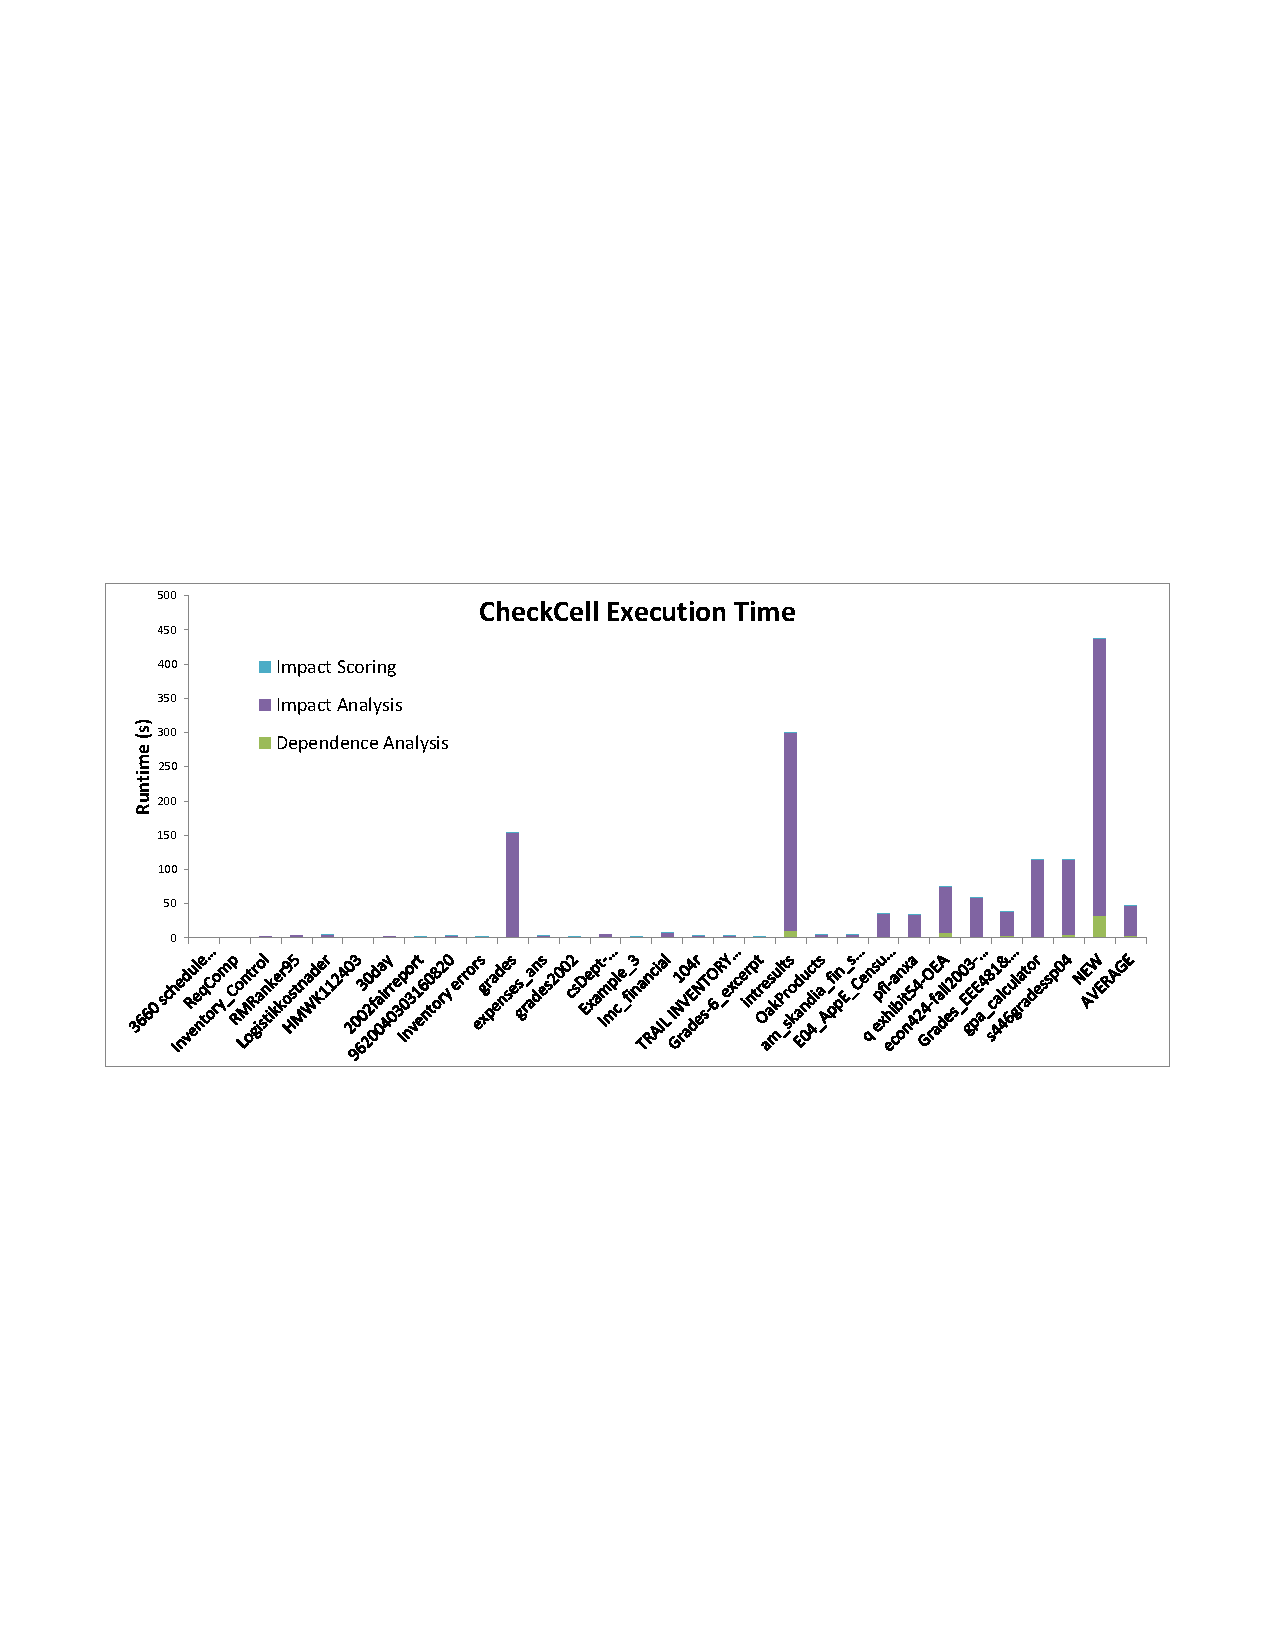
\includegraphics[width=5in]{execution_time_graph}
  \caption{\checkcell{} execution time. For most of the spreadsheets, \checkcell{} completes its analysis in under 9 seconds; for all but two, it completes in under three minutes (see Section~\ref{sec:execution_time}).\label{fig:execution_time_graph}}
\end{figure*}
 
Figure~\ref{fig:execution_time_graph} reports the performance of data
debugging across our spreadsheet suite, ordered by the weighted number
of cells. Table~\ref{tab:spreadsheet_breakdown} includes the full data.

For 19 of the 30 spreadsheets, \checkcell{} takes 9 seconds or less to
complete. Its runtime is less than three minutes for all but two of
the spreadsheets: \texttt{intresults} and \texttt{NEW}, which take 318
seconds and 683 seconds, respectively. The average runtime over all
spreadsheets is 61 seconds; without the two outliers, it is 29
seconds. As our analysis in Section~\ref{sec:asymptotic_analysis}
predicts, the cost of \checkcell{} is generally proportional to the
cost of the impact analysis, which is in turn dependent on the
weighted number of cells.

The two outlier spreadsheets have by far the largest number of formulas
(1,066 and 2,626), and the latter also has the largest number of
weighted cells (2,403). Their relatively high execution time is
attributable to the fact that cost of impact analysis increases as the
number of formulas increases, since the Excel recalculation engine
must do more work per item tested.

\paragraph{Summary:} For nearly every spreadsheet
 examined, \checkcell{}'s runtime is under three minutes; we believe
 this overhead is acceptable for an error detection tool.

% Info about the benchmarks.

% \subsection{Benchmarks}

%\subsection{Case Studies}

% \paragraph{9-Grades}

\subsection{User Study}
\label{sec:user_study}

While \checkcell{} can be used across the EUSES suite, looking for
errors in existing spreadsheets is problematic because we do not know
what the ground truth is. To evaluate \checkcell{}'s efficacy at
finding actual errors, we need errors and ground truth to compare it
against.

We designed an experiment that allows us to observe real errors
produced by people and use \checkcell{} to find them. This experiment
consists of a user study. We collect human errors by hiring workers to
perform data entry tasks (entering known data) via Amazon's Mechanical
Turk, a popular crowdsourcing platform. and then check their results
with \checkcell{}.

Our ground truth data was drawn from \texttt{3q2000.xls}, a
spreadsheet from the EUSES repository that contains selected financial
information from Fannie Mae. We saved the data as a comma-separated
value file (.csv). Mechanical Turk workers were then paid 3 cents to
enter 10 of these values at a time into a web form designed to look
like a spreadsheet, shown in Figure~\ref{fig:mturk_task}. To prevent
copying and pasting, we generate an image containing the
comma-separated values.  Each worker had the opportunity to perform up
to seven different tasks.

In all, we collected 200 responses from 46 distinct users. Out of
these responses, 14 had omitted data and 52 contained errors, for an
overall error rate of 33\%.

We then inserted the erroneous data back into the spreadsheet one at a
time and ran \checkcell{} to see whether it found any of these
errors. Recall that by design, \checkcell{} reports data with an
unusual impact on any of the calculations. For this
spreadsheet, \checkcell{} always highlights the values in the top row
(the net interest income) because these values have a significant
impact on the spreadsheet; most of the income in this spreadsheet
comes from this row. We classify \checkcell{} as having correctly
found an error if it also highlights an erroneous cell.

For 11 of the 52 erroneous inputs (21\%), \checkcell{} correctly marks the
cell with the error, verifying our hypothesis that locating data with
unusual impact also finds errors.


\begin{figure*}[!t]
\centering
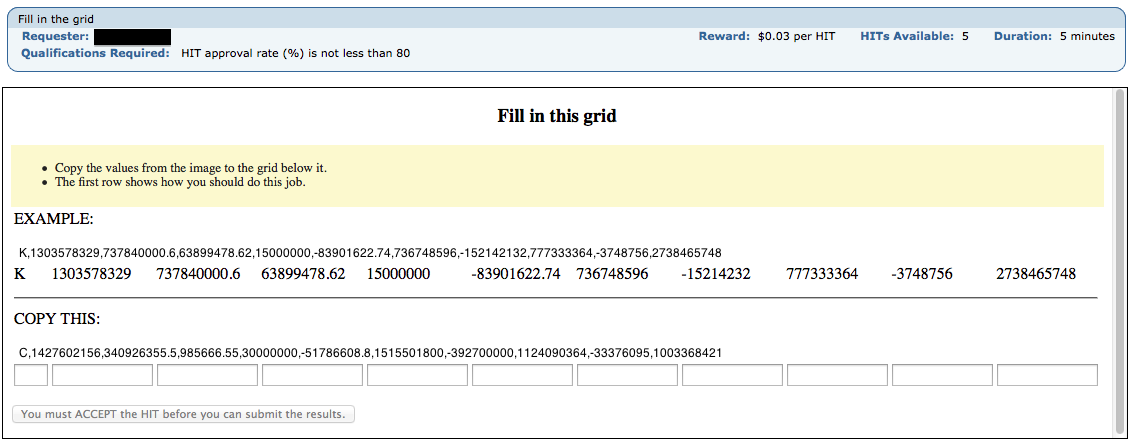
\includegraphics[width=5in]{images/mturk_fuzz_task}
  \caption{The page presented to Mechanical Turk workers to perform data entry tasks in order to collect actual human data entry errors (see Section~\ref{sec:user_study}).\label{fig:mturk_task}}
\end{figure*}


\begin{figure*}[!t]
\centering
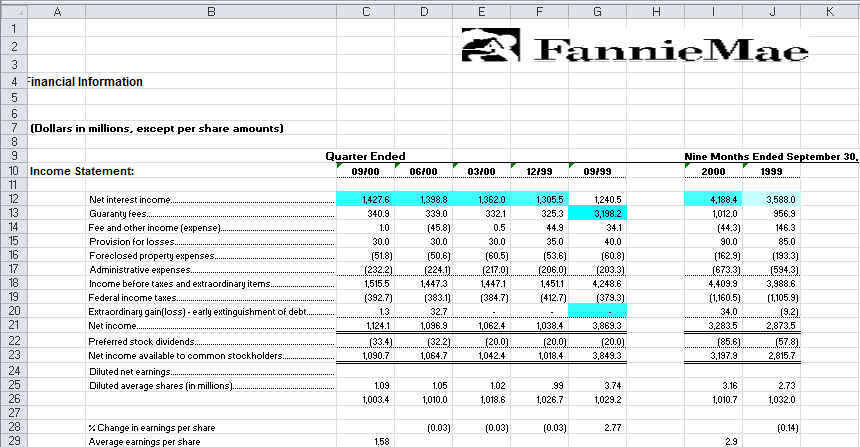
\includegraphics[width=5in]{images/fannie_mae_outlier}
  \caption{A screenshot of \checkcell{}'s results. In addition to the top row, which has a large impact on the final results, \checkcell{} highlights cell \texttt{G19}, a human data entry error.\label{fig:fannie_mae}}
\end{figure*}


Figure~\ref{fig:fannie_mae} presents a screenshot of \checkcell{}'s
results with one of these errors. In addition to the top
row, \checkcell{} indicates that cell \texttt{G19} has an unusual
impact; this is, in fact, the error. The correct value
for \texttt{G19} is \texttt{-379300000}, and the value entered by the
worker was \texttt{3793000000}: the worker made both a sign error and
an order of magnitude error (one too many 0's).

We manually inspected the remaining errors and found that none
have any unusual impact on the spreadsheet's results.

\paragraph{Summary:} By searching for data with unusual impacts on the spreadsheet, \checkcell{} is able to successfully find actual human data entry errors.

